\section{Results}
\label{sec:results}

\subsection{Quantitative Results}

Given the small pilot sample ($N=3$), we report descriptive statistics and preliminary trends rather than inferential statistical claims.

\textbf{Clarity:} Both conditions were rated highly for clarity (Scripted: $M=4.67, SD=0.33$; Adaptive: $M=4.33, SD=0.67$). The scripted version had a slight advantage, likely due to its predictability.

\textbf{Comfort:} Ratings were comparable across conditions (Scripted: $M=4.33, SD=0.67$; Adaptive: $M=4.00, SD=0.82$). Both systems were perceived as comfortable environments for stretching.

\textbf{Adaptability:} In our small sample, the adaptive system received higher ratings ($M=4.33, SD=0.67$) than the scripted system ($M=2.00, SD=0.82$), indicating a strong preliminary trend in favor of context-sensitive guidance.

\textbf{Trust:} Trust ratings were similar between conditions (Scripted: $M=4.33, SD=0.67$; Adaptive: $M=4.00, SD=0.82$), suggesting that the verification loop and safety measures effectively maintained user confidence.

\textbf{Naturalness:} The adaptive system was rated slightly higher for naturalness (Adaptive: $M=4.33, SD=0.33$; Scripted: $M=3.67, SD=0.89$), indicating better human-like interaction.

\textbf{Object Relevance:} In the adaptive condition, object suggestions were rated as highly relevant ($M=4.67, SD=0.33$), demonstrating the effectiveness of the KG-LLM integration.

\begin{figure*}[t]
\centering
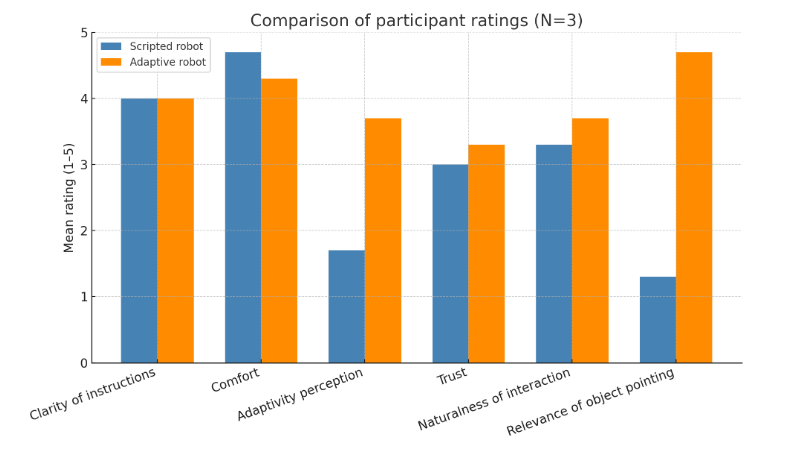
\includegraphics[width=0.88\textwidth]{../images/figure3_results.png}
\caption{Comparative results between scripted and adaptive conditions across the main user-evaluation dimensions.}
\label{fig:comparative_results}
\end{figure*}

Figure~\ref{fig:comparative_results} visualizes the rating profile of both conditions and highlights the same trend observed in the numerical analysis: the adaptive system clearly outperforms the scripted baseline on \textit{adaptivity perception} and \textit{relevance of object pointing}, while \textit{clarity} and \textit{comfort} remain similar or slightly in favor of the scripted mode. This pattern supports our main claim that adaptation improves contextual relevance, but does not automatically guarantee a smoother interaction experience.

\subsection{Response Latency}

Average task completion time was similar between conditions (Scripted: $M=487s, SD=31s$; Adaptive: $M=512s, SD=58s$), with the adaptive system taking slightly longer due to LLM reasoning overhead. In this pilot setting, the observed latency remained within acceptable ranges (mean latency per response: $\approx2$–$3$ seconds).

\subsection{Qualitative Findings}

\textbf{Preference:} Two participants (P2, P3) preferred the scripted version, citing predictability, smoother flow, and lower cognitive load. One participant (P1) preferred the adaptive version, appreciating its personalization and environmental awareness.

\textbf{Strengths of Adaptive System:} Participants noted that the adaptive system was ``more thoughtful,'' ``better at understanding my needs,'' and ``made me feel heard.'' P1 specifically appreciated the robot's suggestion to point to the water bottle when noticing signs of dehydration.

\textbf{Strengths of Scripted System:} The scripted version was perceived as ``more natural and smooth,'' with ``no delays,'' and ``easier to follow.'' Participants appreciated not having to answer questions or make decisions mid-routine.

\textbf{Limitations of Adaptive System:} P2 and P3 reported that ``too many decisions made the session less relaxing,'' and that they ``wanted to just follow along without thinking.'' There were occasional instances where LLM responses seemed slightly off-topic or required clarification.

\textbf{Safety and Trust:} All participants felt safe in both conditions. The verification loop was not explicitly noticed but appeared to prevent problematic suggestions.

Across interviews, qualitative evidence clarified why ratings diverged between conditions. Participants describing the adaptive system as ``more thoughtful'' and ``made me feel heard'' associated these impressions with context-specific recommendations and object-aware prompts, suggesting that adaptation improved perceived relevance. By contrast, participants preferring the scripted mode emphasized flow continuity (``more natural and smooth'') and reduced decision burden (``easier to follow''), indicating that adaptivity can also introduce interaction friction when users expect a low-cognitive-load routine. This trade-off between contextual intelligence and interaction smoothness is a central outcome of the pilot.

\subsection{Technical Observations}

\begin{itemize}
\item \textbf{KG vs. ConceptNet:} In 68\% of reasoning cycles, the response was grounded in the internal KG; in 32\%, ConceptNet was queried. This suggests that custom domain knowledge is valuable but that fallback to general commonsense is necessary for unseen entities.

\item \textbf{LLM Verification Rate:} The secondary verification model corrected or refined 12\% of primary LLM outputs, mostly to adjust tone or clarify action prefixes.

\item \textbf{Multimodal Fusion Robustness:} The fusion of three emotion detection modalities proved robust; even when one modality (e.g., facial recognition due to occlusion) failed, the other two maintained reliable estimates.

\item \textbf{Safety Triggers:} No safety incidents occurred. The emergency stop was never triggered; however, joint limit checks prevented 3 out-of-bounds trajectory commands during the adaptive sessions.
\end{itemize}
